\lstdefinestyle{basherror}{
  language=bash,
  showspaces=false,
  showstringspaces=false,
  breaklines=true,
  postbreak=\mbox{\textcolor{red}{$\hookrightarrow$}\space},
  basicstyle= \small \ttfamily
}


This document collects notes about the HSC PDR1 reprocessing in cycle S18.

Background information can be found in the notes of S17B HSC PDR1 reprocessing (\url{https://confluence.lsstcorp.org/display/DM/S17B+HSC+PDR1+reprocessing}).
The nominal ticket for the S18 PDR1 run is \jira{DM-13666}.
The output repos are:
\begin{enumerate}
\item
/datasets/hsc/repo/rerun/DM-13666/UDEEP/
\item
/datasets/hsc/repo/rerun/DM-13666/DEEP/
\item
/datasets/hsc/repo/rerun/DM-13666/WIDE/
\end{enumerate}

\section{Input dataset}
HSC SSP PDR1 data, as described in \citeds{DMTR-31} Section 1; this is the same as S17B HSC PDR1 reprocessing.
It includes 5654 visits in 7 bands and 3 layers (386 visits in UDEEP, 668 visits in DEEP, and 4600 visits in WIDE).
It has 11 tracts in UDEEP, 37 tracts in DEEP, and 91 tracts in WIDE.

The tract IDs can be found in \url{https://hsc-release.mtk.nao.ac.jp/doc/index.php/database/} (except tract 9572) or the first table on the S17B HSC PDR1 reprocessing page.
The calibration repo is version \texttt{20180117}, located at \texttt{/datasets/hsc/calib/20180117}  (from \jira{DM-13387})

\section{Software stack version}
The processing will use stack version \texttt{w\_2018\_15} (released 2018-04-16).
For verification, the RC2 reprocessing of \texttt{w\_2018\_14} is at \jira{DM-13890} and the RC2 reprocessing of \texttt{w\_2018\_15} is at \jira{DM-14123}.
Pipeline steps and execution units
\begin{enumerate}
\item \texttt{makeSkyMap.py}:   One SkyMap for the whole campaign
\item \texttt{singleFrameDriver.py}:   independent per ccd, typically run per visit
\item \texttt{skyCorrection.py}:   per visit
\item \texttt{mosaic.py}:   per tract x filter, including all visits overlapping that tract in that filter.
\item \texttt{coaddDriver.py}: independent per patch, run per tract x filter, including all overlapping visits
\item \texttt{multiBandDriver.py}:   independent per patch, may run per tract, including all filters
\end{enumerate}
Data of different layers (DEEP/UDEEP/WIDE) are processed separately.

\section{Pipeline configurations}
The HSC default config will be used.
Bad amplifiers are present in ccd 9 therefore it is not processed since results are not trustworthy even if \texttt{processCcd.py} passes.


Operational configurations can be different from the stack defaults; e.g. can make \newline \texttt{config.assembleCoadd.subregionSize} small enough so a full stack of images can fit into memory at once; a trade-off between memory and i/o but doesn't matter scientifically, as the pixels are independent.
Also, pipe\_drivers jobs can be continued with the \texttt{--reuse-outputs-from all} option, rather than starting over.

\section{Reproducible Failures}
In \texttt{singleFrameDriver}/\texttt{processCcd}, there were reproducible failures in 14 CCDs in the UDEEP layer, 6 CCDs in the DEEP layer, and 120 CCDs in the WIDE layer.
The Data IDs that reproducibly caused failures for WIDE are in table-\ref{WIDEFailsTable}, UDEEP in table-\ref{UDEEPFailsTable} and for DEEP in table-\ref{DEEPFailsTable}.

\clearpage
\begin{table}[H]
\centering
\begin{tabular} {|c|c||c|c|}
\hline
visit & ccd & visit & ccd \\
\hline
6342 & 11, 99, 24, 59, 67, 75, 96 & 34332 & 61     \\      
13166 & 20                        & 35852 & 8      \\       
13178 & 91                        & 35862 & 61     \\      
13182 & 101                       & 35882 & 19     \\      
13198 & 84, 85, 90, 91            & 35892 & 12     \\      
13288 & 84                        & 35894 & 86     \\      
15096 & 47, 54                    & 35908 & 28     \\      
16064 & 101                       & 35916 & 50     \\      
17670 & 24                        & 35942 & 4, 64  \\   
17672 & 24                        & 35948 & 72     \\      
17692 & 7, 8                      & 35966 & 60     \\      
17722 & 20                        & 36178 & 98     \\      
17736 & 63                        & 36216 & 6      \\       
17738 & 69                        & 36264 & 94     \\      
17750 & 58                        & 36604 & 81     \\      
19394 & 24                        & 37532 & 33     \\      
19414 & 8                         & 37538 & 100    \\     
19454 & 20                        & 37552 & 12     \\      
19468 & 69                        & 37988 & 33     \\      
19646 & 2                         & 38316 & 11     \\      
25894 & 68                        & 38328 & 91     \\      
25956 & 76                        & 38330 & 8      \\       
25968 & 65                        & 38346 & 8      \\       
26054 & 43                        & 38912 & 86     \\      
27068 & 96                        & 42218 & 102    \\     
29378 & 70                        & 42222 & 102    \\     
29898 & 99                        & 42454 & 17, 24 \\  
29916 & 99                        & 42510 & 77     \\      
29936 & 66                        & 42534 & 65     \\      
29942 & 96                        & 44050 & 94     \\      
29966 & 103                       & 44060 & 31     \\      
30588 & 98                        & 44090 & 27     \\      
31410 & 73                        & 44154 & 66     \\      
32506 & 3, 8                      & 44160 & 55     \\      
33824 & 56                        & 44162 & 61     \\      
33862 & 8                         & 45262 & 64     \\      
33890 & 61                        & 45348 & 64     \\      
33934 & 95                        & 45940 & 47     \\      
33950 & 52, 60                    & 46892 & 64     \\      
34268 & 103                       &       &        \\
\hline
\end{tabular}
\caption{IDs of WIDE ccds with reproducible failures.}
\label{WIDEFailsTable}
\end{table} 

\begin{table}[ht]
\centering
\begin{tabular} {|c|c|}
\hline
visit & ccd \\
\hline
17934 & 1 \\
19712 & 33 \\
23596 & 6 \\
37828 & 101 \\
38494 & \begin{tabular}[x]{@{}c@{}} 4, 6, 11, 32, 37, 43, \\ 54, 80, 96, 102 \end{tabular} \\
\hline
\end{tabular}
\caption{IDs of UDEEP ccds with reproducible failures}
\label{UDEEPFailsTable}
\end{table}

\begin{table}[ht]
\centering
\begin{tabular} {|c|c|}
\hline
visit & ccd \\
\hline
19702 & 12 \\
22640 & 10 \\
24342 & 102 \\
9664  & 94 \\
36842 & 94 \\
15206 & 100 \\
\hline
\end{tabular}
\caption{IDs of DEEP ccds with reproducible failures.}
\label{DEEPFailsTable}
\end{table}


Out of the 140 failures:
\begin{enumerate}
\item 58 failed with \lstinline[style=basherror]+Unable to match sources!+
\item 31 failed with \lstinline[style=basherror]+No matches to use for photocal+
\item 12 failed with \lstinline[style=basherror]+No objects passed our cuts for consideration as psf stars+
\item 2 failed with
    \begin{lstlisting}[style=basherror]
    Unable to measure aperture correction for required algorithm 'modelfit\_CModel\_exp': only [01] sources, but require at least 2.
    \end{lstlisting}
\item 37 failed with
    \begin{lstlisting}[style=basherror]
    InvalidParameterError: 'Only spatial variation (ndim == 2) is supported; saw 0'" which trace back to "PSF star selector found [123] candidates" in processCcd.charImage.measurePsf
    \end{lstlisting}
\end{enumerate}

Rerun logs of these failures are attached in \jira{DM-13667}.
In \texttt{coaddDriver}, there were no FATAL- or ERROR-level log records, but many WARN-level records.
Among them there were three kinds of "errors" in edge patches:
\begin{enumerate}
\item \lstinline[style=basherror]+CoaddDriver IndexError: cannot do a non-empty take from an empty axes+ (see \jira{DM-14282}) appears in 8 patches:
\begin{table}[h]
\centering
\begin{tabular} {|c|c|c|c|}
\hline
Layer & Filter & Tracts  & Patches  \\
\hline

\multirow{2}{*}{UDEEP} & HSC-G                  & 8766  & 8,3 \\ \cline{2-4}
                       & HSC-Y                  & 9571  & 7,7 \\ \hline
\multirow{5}{*}{DEEP}  & \multirow{2}{*}{HSC-G} & 9708  & 7,6 \\ \cline{3-4}
                       &                        & 9812  & 7,7 \\ \cline{2-4}
                       & \multirow{2}{*}{HSC-I} & 8766  & 0,5 \\ \cline{3-4}
                       &                        & 9707  & 6,6 \\ \hline
WIDE                   & HSC-G                  & 16972 & 0,7 \\
\hline
\end{tabular}
\caption{Dataset IDs where IndexError was encountered.}
\label{table1}
\end{table}

\item \lstinline[style=basherror]+CompareWarpAssembleCoadd RuntimeError: No PsfMatched warps were found+ (see \jira{DM-14286}) edge cases when no \texttt{psfMatchedWarp} files were written because there were 0 good pixels appears in 5 patches:
\begin{table}[h]
\centering
\begin{tabular} {|c|c|c|c|}
\hline
Layer & Filter & Tracts  & Patches  \\
\hline

\multirow{4}{*}{DEEP}  & NB0816                 & 9463                   & 7,0 \\ \cline{2-4}
                       & \multirow{2}{*}{HSC-Z} & 8525                   & 1,5 \\ \cline{3-4}
                       &                        & \multirow{2}{*}{9465}  & 5,6 \\
                       &                        &                        & 4,8 \\ \hline
WIDE                   & HSC-I                  & 16821                  & 2,6 \\
\hline
\end{tabular}
\caption{Dataset IDs where RuntimeError was encountered.}
\label{RuntimeErrorsTable}
\end{table}

\item \lstinline[style=basherror]+DetectCoaddSources RuntimeError: Variance rescaling factor exceeds configured limit+ (see \jira{DM-14303}) occurs at 1 edge patch in \texttt{HSC-I} of \texttt{WIDE} layer on tract \texttt{9940} and patch \texttt{3,8}.
\end{enumerate}

\section{Compute resource}
A slrum reservation is made for this reprocessing campaign (\jira{IHS-749}).
Outputs will be stored in GPFS \texttt{/datasets/}   (\jira{IHS-914}, \jira{IHS-954}).
The numbers of Slurm Jobs are listed in Table \ref{table1}.
Slurm Job IDs can be found in the files attached on \url{https://confluence.lsstcorp.org/display/DM/S18+HSC+PDR1+reprocessing}.
Only jobs that contributed to the archived data products.
\begin{table}
\centering
\begin{tabular} {|c|c|c|c|}
\hline
pipeline & UDEEP & DEEP & WIDE \\
\hline
makeSkyMap & 1 & 1 & 1 \\
singleFrameDriver&1 & 7 & 149 \\
skyCorrection&1 & 7 & 149 \\
mosaic&69 & 218 & 455 \\
coaddDriver&69 & 218 & 455 \\
multiBandDriver &11+1 \footnote{tract=9813 was continued with reuse} & 37 & 91 \\
\hline
\end{tabular}
\caption{Number of Slurm Jobs}
\label{table1}
\end{table}

The node-hours usage based on Slurm accounting is listed in Table \ref{table2}.
In order to create these plots and collect the information for the table below, \texttt{usage.py} from \url{https://github.com/lsst-dm/ldf_ops_tools/tree/master/usage} was used.
It should be noted that since the node-hours are rounded to two decimal places, the total node hours might be slightly off from what would be found if the individual code node-hours were summed.
\begin{table}
\centering
\begin{tabular} {|c|c|c|c|c|}
\hline
pipeline & UDEEP & DEEP & WIDE & Total\\
\hline
makeSkyMap&0.02& 0.02& 0.02& 0.07\\
singleFrameDriver&61.48& 110.14& 1163.02& 1334.63\\
skyCorrection&3.99& 6.55& 51.45& 61.99\\
mosaic&15.52& 24.67& 139.18& 179.37\\
coaddDriver&118.63& 185.49& 803.40& 1107.53\\
multiBandDriver&795.48& 1186.90& 4561.18&6543.57\\
\hline
Total node hours&995.12&1513.78&6718.25&9227.15\\
\hline
\end{tabular}
\caption{Node-hours usage from Slurm accounting rounded to two decimal places}
\label{table2}
\end{table}


\begin{figure}[ht]
    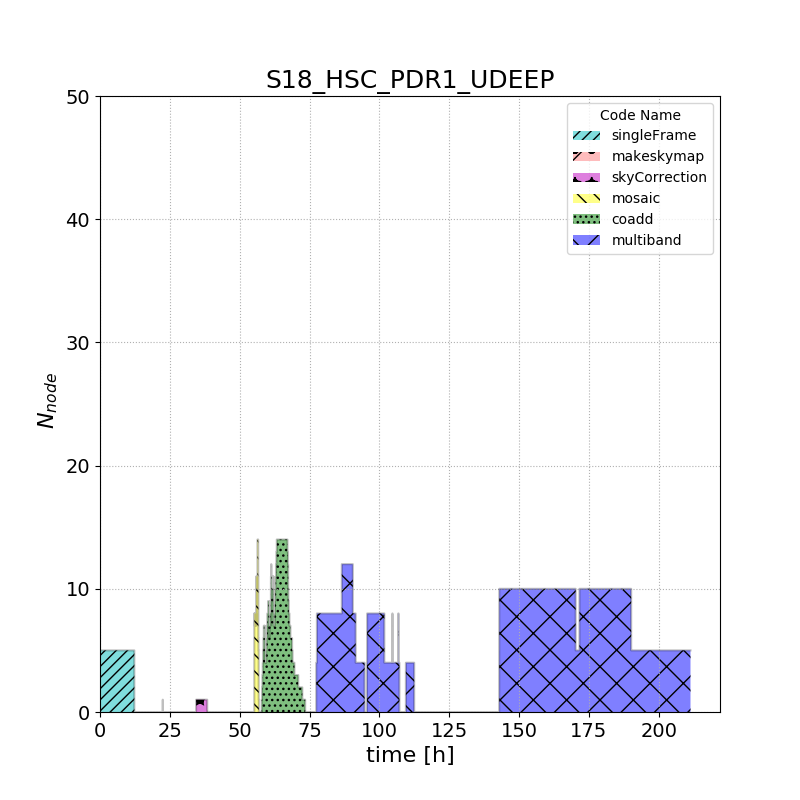
\includegraphics[width=0.50\textwidth]{usage-S18_HSC_PDR1_UDEEP.png}
    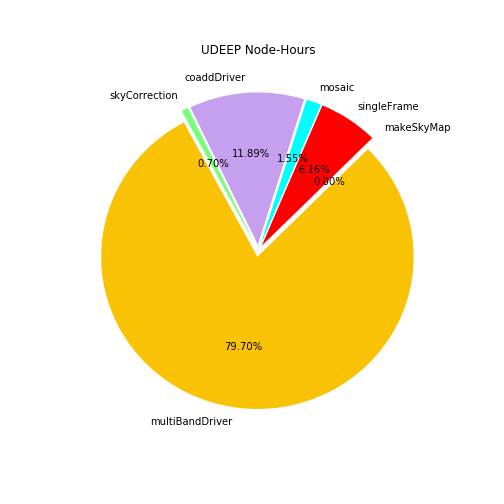
\includegraphics[width=0.50\textwidth]{PDR1_UDEEP_pie.png}
    \caption{Node-hours usage from Slurm accounting. The UDEEP layer.}
    \label{UDEEPslurm}
\end{figure}

\begin{figure}[ht]
    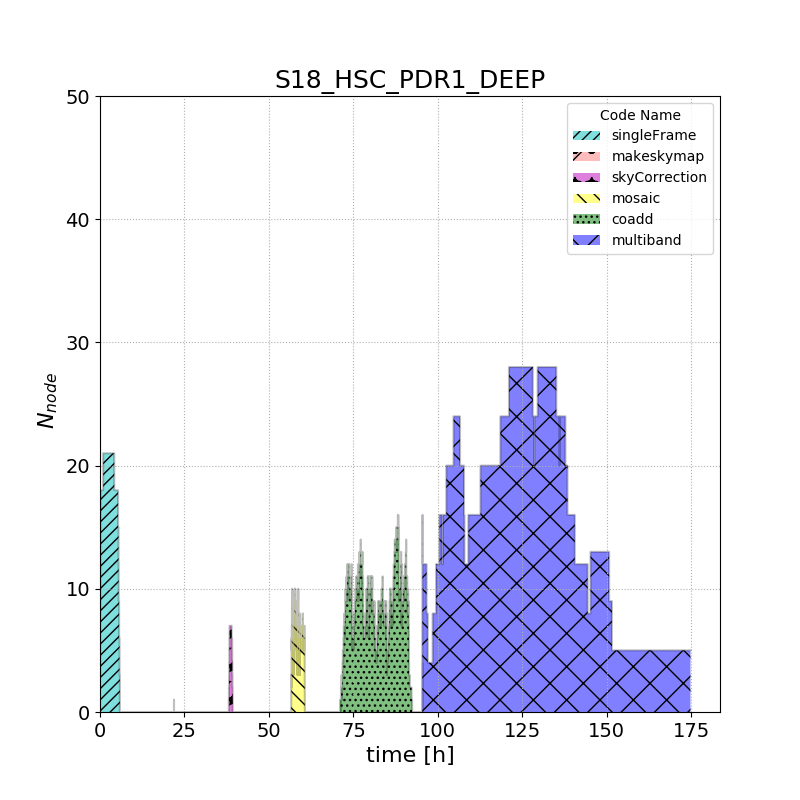
\includegraphics[width=0.50\textwidth]{usage-S18_HSC_PDR1_DEEP.png}
    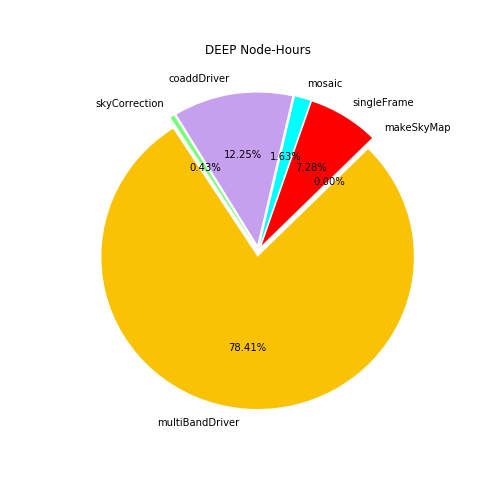
\includegraphics[width=0.50\textwidth]{PDR1_DEEP_pie.png}
    \caption{Node-hours usage from Slurm accounting. The DEEP layer.}
    \label{DEEPslurm}
\end{figure}

\begin{figure}[ht]
    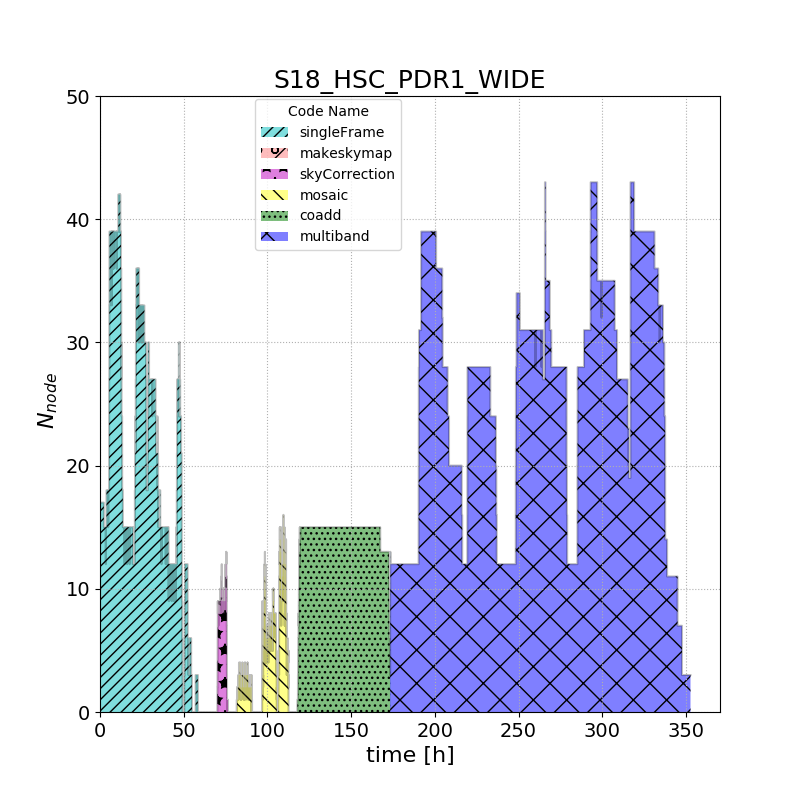
\includegraphics[width=0.50\textwidth]{usage-S18_HSC_PDR1_WIDE.png}
    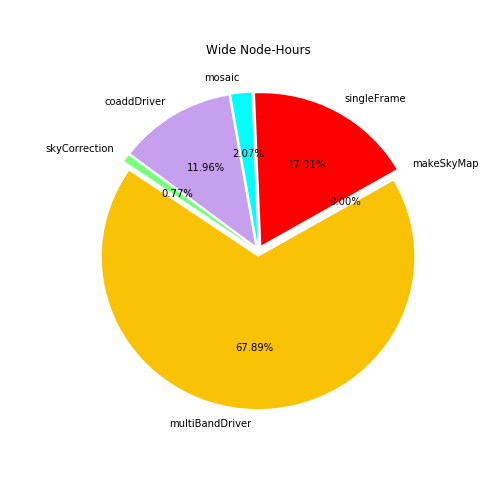
\includegraphics[width=0.50\textwidth]{PDR1_Wide_pie.png}
    \caption{Node-hours usage from Slurm accounting. The WIDE layer.}
    \label{WIDEslurm}
\end{figure}

\begin{figure}[ht]
    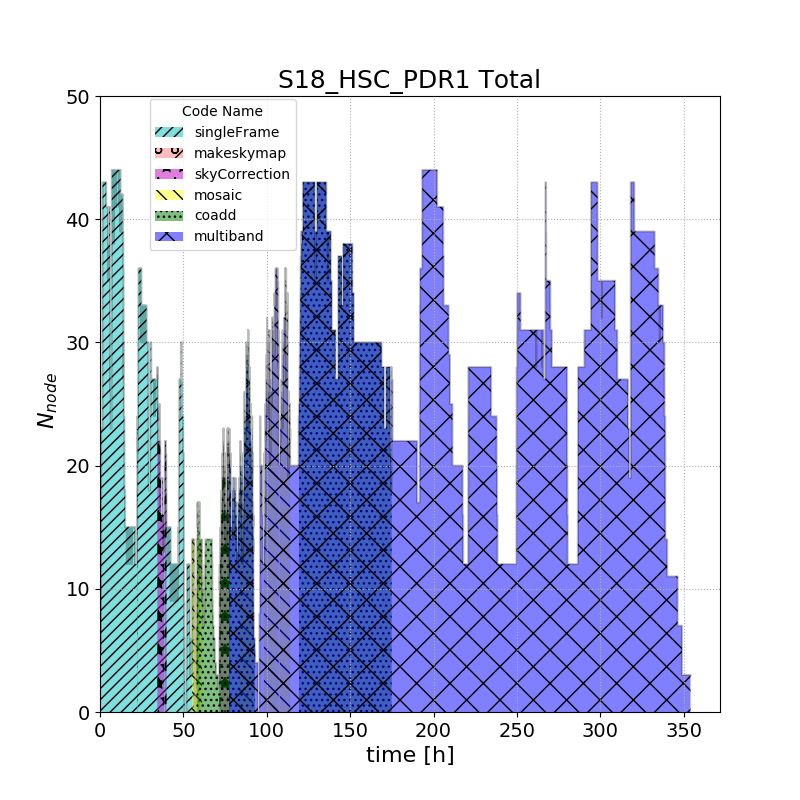
\includegraphics[width=0.50\textwidth]{usage-S18_HSC_PDR1_Total.png}
    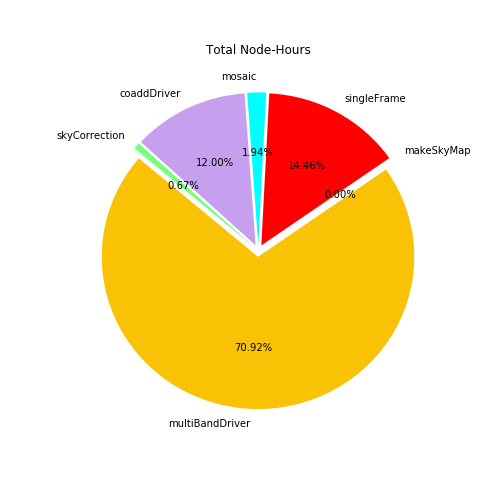
\includegraphics[width=0.50\textwidth]{PDR1_Total_pie.png}
    \caption{Total node-hours usage from Slurm accounting}
    \label{TOTslurm}
\end{figure}

\section{Low-level processing details}
This section includes low-level details that may only be of interest to the operation team.
The first \texttt{singleFrameDriver} job that contributed to the output data products started on April 20, the last multiband job finished on May 5.

In the beginning we attempted to run each visit as its own \texttt{singleFrameDriver}.
One advantage of doing so is that each visit would have its own log file.
During the attempt, many jobs took much longer than expected and timed out.
The IO wait time on GPFS was excessively high (e.g. \approx5 sec), likely because too many nodes simultaneously put locks on the same folders and sometimes same files.
So we changed the strategy, and grouped multiple visits into fewer \texttt{singleFrameDriver} calls.
The modified strategy was then to group all UDEEP visits into one singleFrameDriver job, DEEP visits into 7 jobs, and WIDE visits into 149 jobs.

Each of the grouped \texttt{singleFrameDriver} used multiple nodes.
A non-small percentage (~30\%) of jobs failed at slurm failing to launch the job.
This is after \texttt{singleFrameDriver.py} successfully submitted the job to slurm, the job waited in the queue for its turn, and the job started trying once it got its turn, but then the job failed to launch with a message about socket timeout.
This failure wasn't restricted to one specific worker node.
 
\jira{DM-14181} was filed for further investigations.
All failures were resubmitted iteratively, with many failed again in the iterations, and eventually were all pushed though.
On Apr 24 morning, the verification cluster used a brief downtime and the LDAP timeout in sssd.conf was increased on verify nodes.
Afterwards the socket timeout problems were no longer seen.

The execution of \texttt{skyCorrection.py} is independent per visit.
The visit grouping of \texttt{singleFrameDriver} was used, resulting in 157 slurm jobs.

A sqlite3 file was made for each layer to store information of what tract/patch overlaps what ccds, checking through each calexp using skymap.findTractPatchList  and geom.convexHull features.
Different from the S17B HSC PDR1 reprocessing, only tracts that are in the PDR1 were included this time; the tract IDs can be found in \url{https://hsc-release.mtk.nao.ac.jp/doc/index.php/database/} (except tract 9572) or the first table on the S17B HSC PDR1 reprocessing page (\url{https://confluence.lsstcorp.org/display/DM/S17B+HSC+PDR1+reprocessing}).
A few additional tracts were processed in the first place but were manually cleaned up afterwards.

For each tract and filter combination \texttt{mosaic.py} and \texttt{coaddDriver.py} were run, using all visits overlapping that tract in that filter for each layer, i.e. 69 jobs in UDEEP, 218 jobs in DEEP, and 455 jobs in WIDE.
A single node was used for each job.

After which \texttt{multiBandDriver.py} was then run for each tract.  There are 11 tracts in total in the UDEEP layer, so the starting plan was to run multiband in 11 jobs.
In the first attempt, each used 4 nodes and 12 cores per node.
Some jobs failed to launch due to \jira{DM-14181}, before the sssd timeout window was updated on Apr 24 morning.
Those jobs were resubmitted.
Some jobs failed because they went out of memory; they were tract 8523 and tract 9813.
I then attempted to run them with 5 nodes and 6 cores each (without reusing the existing data).
Increasing resources resulted with tract 8523 finishing but tract 9813 went out of memory again.
I continued tract 9813 using the \texttt{--reuse-outputs-from option}, and then it completed.
Therefore, 12 slurm jobs in total contributed to the output data products in UDEEP.


In the DEEP layer, there are 37 tracts in total.
In the first attempt, 37 slurm jobs were submitted and each used 4 nodes and 12 cores.
All completed except the job of tract 9463 went out of memory and failed.
Re-running using 5 nodes and 6 cores each, without reusing the existing data, completed tract 9463.
In the WIDE layer, there are 91 tracts in total.
It was completed in 91 slurm jobs, using either 4 or 3 nodes per job, 12 cores per node.

In many cases, we set a larger time limit or allowed more memory than strictly necessary; this was not optimal but helped minimizing manual intervention throughout the campaign, arguably improving the overall throughput.

The campaign mainly used the 15 worker nodes under the slurm reservation (\jira{IHS-749}) but also used other workers outside of the reservation if they were idle.
Throughout the campaign, we did not occupy the entire cluster and at least some worker nodes in the normal queue were available for or used by other users.
The intention was to allow developers to bypass the production jobs for their small jobs (a few nodes) and in a short queue for large jobs.
This balance was kept manually.
 It would be nice to have a production queue doing this for me (and also have a more consistent balance).

